
%% bare_conf.tex
%% V1.4
%% 2012/12/27
%% by Michael Shell
%% See:
%% http://www.michaelshell.org/
%% for current contact information.
%%
%% This is a skeleton file demonstrating the use of IEEEtran.cls
%% (requires IEEEtran.cls version 1.8 or later) with an IEEE conference paper.
%%
%% Support sites:
%% http://www.michaelshell.org/tex/ieeetran/
%% http://www.ctan.org/tex-archive/macros/latex/contrib/IEEEtran/
%% and
%% http://www.ieee.org/

%%*************************************************************************
%% Legal Notice:
%% This code is offered as-is without any warranty either expressed or
%% implied; without even the implied warranty of MERCHANTABILITY or
%% FITNESS FOR A PARTICULAR PURPOSE! 
%% User assumes all risk.
%% In no event shall IEEE or any contributor to this code be liable for
%% any damages or losses, including, but not limited to, incidental,
%% consequential, or any other damages, resulting from the use or misuse
%% of any information contained here.
%%
%% All comments are the opinions of their respective authors and are not
%% necessarily endorsed by the IEEE.
%%
%% This work is distributed under the LaTeX Project Public License (LPPL)
%% ( http://www.latex-project.org/ ) version 1.3, and may be freely used,
%% distributed and modified. A copy of the LPPL, version 1.3, is included
%% in the base LaTeX documentation of all distributions of LaTeX released
%% 2003/12/01 or later.
%% Retain all contribution notices and credits.
%% ** Modified files should be clearly indicated as such, including  **
%% ** renaming them and changing author support contact information. **
%%
%% File list of work: IEEEtran.cls, IEEEtran_HOWTO.pdf, bare_adv.tex,
%%                    bare_conf.tex, bare_jrnl.tex, bare_jrnl_compsoc.tex,
%%                    bare_jrnl_transmag.tex
%%*************************************************************************

% *** Authors should verify (and, if needed, correct) their LaTeX system  ***
% *** with the testflow diagnostic prior to trusting their LaTeX platform ***
% *** with production work. IEEE's font choices can trigger bugs that do  ***
% *** not appear when using other class files.                            ***
% The testflow support page is at:
% http://www.michaelshell.org/tex/testflow/



% Note that the a4paper option is mainly intended so that authors in
% countries using A4 can easily print to A4 and see how their papers will
% look in print - the typesetting of the document will not typically be
% affected with changes in paper size (but the bottom and side margins will).
% Use the testflow package mentioned above to verify correct handling of
% both paper sizes by the user's LaTeX system.
%
% Also note that the "draftcls" or "draftclsnofoot", not "draft", option
% should be used if it is desired that the figures are to be displayed in
% draft mode.
%
\documentclass[conference]{IEEEtran}
% Add the compsoc option for Computer Society conferences.
%
% If IEEEtran.cls has not been installed into the LaTeX system files,
% manually specify the path to it like:
% \documentclass[conference]{../sty/IEEEtran}


\usepackage[utf8]{inputenc}

\usepackage{bigfoot}
\usepackage{hyperref}
\usepackage{graphicx}
\graphicspath{ {./images/} }

% Some very useful LaTeX packages include:
% (uncomment the ones you want to load)


% *** MISC UTILITY PACKAGES ***
%
%\usepackage{ifpdf}
% Heiko Oberdiek's ifpdf.sty is very useful if you need conditional
% compilation based on whether the output is pdf or dvi.
% usage:
% \ifpdf
%   % pdf code
% \else
%   % dvi code
% \fi
% The latest version of ifpdf.sty can be obtained from:
% http://www.ctan.org/tex-archive/macros/latex/contrib/oberdiek/
% Also, note that IEEEtran.cls V1.7 and later provides a builtin
% \ifCLASSINFOpdf conditional that works the same way.
% When switching from latex to pdflatex and vice-versa, the compiler may
% have to be run twice to clear warning/error messages.






% *** CITATION PACKAGES ***
%
%\usepackage{cite}
% cite.sty was written by Donald Arseneau
% V1.6 and later of IEEEtran pre-defines the format of the cite.sty package
% \cite{} output to follow that of IEEE. Loading the cite package will
% result in citation numbers being automatically sorted and properly
% "compressed/ranged". e.g., [1], [9], [2], [7], [5], [6] without using
% cite.sty will become [1], [2], [5]--[7], [9] using cite.sty. cite.sty's
% \cite will automatically add leading space, if needed. Use cite.sty's
% noadjust option (cite.sty V3.8 and later) if you want to turn this off
% such as if a citation ever needs to be enclosed in parenthesis.
% cite.sty is already installed on most LaTeX systems. Be sure and use
% version 4.0 (2003-05-27) and later if using hyperref.sty. cite.sty does
% not currently provide for hyperlinked citations.
% The latest version can be obtained at:
% http://www.ctan.org/tex-archive/macros/latex/contrib/cite/
% The documentation is contained in the cite.sty file itself.






% *** GRAPHICS RELATED PACKAGES ***
%
\ifCLASSINFOpdf
  % \usepackage[pdftex]{graphicx}
  % declare the path(s) where your graphic files are
  % \graphicspath{{../pdf/}{../jpeg/}}
  % and their extensions so you won't have to specify these with
  % every instance of \includegraphics
  % \DeclareGraphicsExtensions{.pdf,.jpeg,.png}
\else
  % or other class option (dvipsone, dvipdf, if not using dvips). graphicx
  % will default to the driver specified in the system graphics.cfg if no
  % driver is specified.
  % \usepackage[dvips]{graphicx}
  % declare the path(s) where your graphic files are
  % \graphicspath{{../eps/}}
  % and their extensions so you won't have to specify these with
  % every instance of \includegraphics
  % \DeclareGraphicsExtensions{.eps}
\fi
% graphicx was written by David Carlisle and Sebastian Rahtz. It is
% required if you want graphics, photos, etc. graphicx.sty is already
% installed on most LaTeX systems. The latest version and documentation
% can be obtained at: 
% http://www.ctan.org/tex-archive/macros/latex/required/graphics/
% Another good source of documentation is "Using Imported Graphics in
% LaTeX2e" by Keith Reckdahl which can be found at:
% http://www.ctan.org/tex-archive/info/epslatex/
%
% latex, and pdflatex in dvi mode, support graphics in encapsulated
% postscript (.eps) format. pdflatex in pdf mode supports graphics
% in .pdf, .jpeg, .png and .mps (metapost) formats. Users should ensure
% that all non-photo figures use a vector format (.eps, .pdf, .mps) and
% not a bitmapped formats (.jpeg, .png). IEEE frowns on bitmapped formats
% which can result in "jaggedy"/blurry rendering of lines and letters as
% well as large increases in file sizes.
%
% You can find documentation about the pdfTeX application at:
% http://www.tug.org/applications/pdftex





% *** MATH PACKAGES ***
%
%\usepackage[cmex10]{amsmath}
% A popular package from the American Mathematical Society that provides
% many useful and powerful commands for dealing with mathematics. If using
% it, be sure to load this package with the cmex10 option to ensure that
% only type 1 fonts will utilized at all point sizes. Without this option,
% it is possible that some math symbols, particularly those within
% footnotes, will be rendered in bitmap form which will result in a
% document that can not be IEEE Xplore compliant!
%
% Also, note that the amsmath package sets \interdisplaylinepenalty to 10000
% thus preventing page breaks from occurring within multiline equations. Use:
%\interdisplaylinepenalty=2500
% after loading amsmath to restore such page breaks as IEEEtran.cls normally
% does. amsmath.sty is already installed on most LaTeX systems. The latest
% version and documentation can be obtained at:
% http://www.ctan.org/tex-archive/macros/latex/required/amslatex/math/





% *** SPECIALIZED LIST PACKAGES ***
%
%\usepackage{algorithmic}
% algorithmic.sty was written by Peter Williams and Rogerio Brito.
% This package provides an algorithmic environment fo describing algorithms.
% You can use the algorithmic environment in-text or within a figure
% environment to provide for a floating algorithm. Do NOT use the algorithm
% floating environment provided by algorithm.sty (by the same authors) or
% algorithm2e.sty (by Christophe Fiorio) as IEEE does not use dedicated
% algorithm float types and packages that provide these will not provide
% correct IEEE style captions. The latest version and documentation of
% algorithmic.sty can be obtained at:
% http://www.ctan.org/tex-archive/macros/latex/contrib/algorithms/
% There is also a support site at:
% http://algorithms.berlios.de/index.html
% Also of interest may be the (relatively newer and more customizable)
% algorithmicx.sty package by Szasz Janos:
% http://www.ctan.org/tex-archive/macros/latex/contrib/algorithmicx/




% *** ALIGNMENT PACKAGES ***
%
%\usepackage{array}
% Frank Mittelbach's and David Carlisle's array.sty patches and improves
% the standard LaTeX2e array and tabular environments to provide better
% appearance and additional user controls. As the default LaTeX2e table
% generation code is lacking to the point of almost being broken with
% respect to the quality of the end results, all users are strongly
% advised to use an enhanced (at the very least that provided by array.sty)
% set of table tools. array.sty is already installed on most systems. The
% latest version and documentation can be obtained at:
% http://www.ctan.org/tex-archive/macros/latex/required/tools/


% IEEEtran contains the IEEEeqnarray family of commands that can be used to
% generate multiline equations as well as matrices, tables, etc., of high
% quality.




% *** SUBFIGURE PACKAGES ***
%\ifCLASSOPTIONcompsoc
%  \usepackage[caption=false,font=normalsize,labelfont=sf,textfont=sf]{subfig}
%\else
%  \usepackage[caption=false,font=footnotesize]{subfig}
%\fi
% subfig.sty, written by Steven Douglas Cochran, is the modern replacement
% for subfigure.sty, the latter of which is no longer maintained and is
% incompatible with some LaTeX packages including fixltx2e. However,
% subfig.sty requires and automatically loads Axel Sommerfeldt's caption.sty
% which will override IEEEtran.cls' handling of captions and this will result
% in non-IEEE style figure/table captions. To prevent this problem, be sure
% and invoke subfig.sty's "caption=false" package option (available since
% subfig.sty version 1.3, 2005/06/28) as this is will preserve IEEEtran.cls
% handling of captions.
% Note that the Computer Society format requires a larger sans serif font
% than the serif footnote size font used in traditional IEEE formatting
% and thus the need to invoke different subfig.sty package options depending
% on whether compsoc mode has been enabled.
%
% The latest version and documentation of subfig.sty can be obtained at:
% http://www.ctan.org/tex-archive/macros/latex/contrib/subfig/




% *** FLOAT PACKAGES ***
%
%\usepackage{fixltx2e}
% fixltx2e, the successor to the earlier fix2col.sty, was written by
% Frank Mittelbach and David Carlisle. This package corrects a few problems
% in the LaTeX2e kernel, the most notable of which is that in current
% LaTeX2e releases, the ordering of single and double column floats is not
% guaranteed to be preserved. Thus, an unpatched LaTeX2e can allow a
% single column figure to be placed prior to an earlier double column
% figure. The latest version and documentation can be found at:
% http://www.ctan.org/tex-archive/macros/latex/base/


%\usepackage{stfloats}
% stfloats.sty was written by Sigitas Tolusis. This package gives LaTeX2e
% the ability to do double column floats at the bottom of the page as well
% as the top. (e.g., "\begin{figure*}[!b]" is not normally possible in
% LaTeX2e). It also provides a command:
%\fnbelowfloat
% to enable the placement of footnotes below bottom floats (the standard
% LaTeX2e kernel puts them above bottom floats). This is an invasive package
% which rewrites many portions of the LaTeX2e float routines. It may not work
% with other packages that modify the LaTeX2e float routines. The latest
% version and documentation can be obtained at:
% http://www.ctan.org/tex-archive/macros/latex/contrib/sttools/
% Do not use the stfloats baselinefloat ability as IEEE does not allow
% \baselineskip to stretch. Authors submitting work to the IEEE should note
% that IEEE rarely uses double column equations and that authors should try
% to avoid such use. Do not be tempted to use the cuted.sty or midfloat.sty
% packages (also by Sigitas Tolusis) as IEEE does not format its papers in
% such ways.
% Do not attempt to use stfloats with fixltx2e as they are incompatible.
% Instead, use Morten Hogholm'a dblfloatfix which combines the features
% of both fixltx2e and stfloats:
%
% \usepackage{dblfloatfix}
% The latest version can be found at:
% http://www.ctan.org/tex-archive/macros/latex/contrib/dblfloatfix/




% *** PDF, URL AND HYPERLINK PACKAGES ***
%
%\usepackage{url}
% url.sty was written by Donald Arseneau. It provides better support for
% handling and breaking URLs. url.sty is already installed on most LaTeX
% systems. The latest version and documentation can be obtained at:
% http://www.ctan.org/tex-archive/macros/latex/contrib/url/
% Basically, \url{my_url_here}.




% *** Do not adjust lengths that control margins, column widths, etc. ***
% *** Do not use packages that alter fonts (such as pslatex).         ***
% There should be no need to do such things with IEEEtran.cls V1.6 and later.
% (Unless specifically asked to do so by the journal or conference you plan
% to submit to, of course. )


% correct bad hyphenation here
\hyphenation{op-tical net-works semi-conduc-tor}


\begin{document}
%
% paper title
% can use linebreaks \\ within to get better formatting as desired
% Do not put math or special symbols in the title.
\title{Smartphone Memory Forensics}


% author names and affiliations
% use a multiple column layout for up to three different
% affiliations
\author{\IEEEauthorblockN{David Andersen}
\IEEEauthorblockA{Gjøvik University College\\
Email: 140409@hig.no}
\and
\IEEEauthorblockN{Tom Roar Furunes}
\IEEEauthorblockA{Gjøvik University College\\
Email: 140467@hig.no}
\and
\IEEEauthorblockN{Geir Haugen}
\IEEEauthorblockA{Gjøvik University College\\
Email: 140464@hig.no}
\and
\IEEEauthorblockN{Torbjørn Jørgensen}
\IEEEauthorblockA{Gjøvik University College\\
Email: 140459@hig.no}
\and
\IEEEauthorblockN{Kevin Mikkelsen}
\IEEEauthorblockA{Gjøvik University College\\
Email: 100889@hig.no}
\and
\IEEEauthorblockN{Sindre Smistad}
\IEEEauthorblockA{Gjøvik University College\\
Email: 140468@hig.no}
\and}

% conference papers do not typically use \thanks and this command
% is locked out in conference mode. If really needed, such as for
% the acknowledgment of grants, issue a \IEEEoverridecommandlockouts
% after \documentclass

% for over three affiliations, or if they all won't fit within the width
% of the page, use this alternative format:
% 
%\author{\IEEEauthorblockN{Michael Shell\IEEEauthorrefmark{1},
%Homer Simpson\IEEEauthorrefmark{2},
%James Kirk\IEEEauthorrefmark{3}, 
%Montgomery Scott\IEEEauthorrefmark{3} and
%Eldon Tyrell\IEEEauthorrefmark{4}}
%\IEEEauthorblockA{\IEEEauthorrefmark{1}School of Electrical and Computer Engineering\\
%Georgia Institute of Technology,
%Atlanta, Georgia 30332--0250\\ Email: see http://www.michaelshell.org/contact.html}
%\IEEEauthorblockA{\IEEEauthorrefmark{2}Twentieth Century Fox, Springfield, USA\\
%Email: homer@thesimpsons.com}
%\IEEEauthorblockA{\IEEEauthorrefmark{3}Starfleet Academy, San Francisco, California 96678-2391\\
%Telephone: (800) 555--1212, Fax: (888) 555--1212}
%\IEEEauthorblockA{\IEEEauthorrefmark{4}Tyrell Inc., 123 Replicant Street, Los Angeles, California 90210--4321}}




% use for special paper notices
%\IEEEspecialpapernotice{(Invited Paper)}




% make the title area
\maketitle

% As a general rule, do not put math, special symbols or citations
% in the abstract
\begin{abstract}
Smart phones today are getting ever more powerful , and capable of doing most of tasks usually associated 
with computers. This have made them increasingly interesting in forensics investigations and information 
theft. In this paper we present the findings we have done when looking at the volatile memory of a virtual 
android device. In our research we have used string search and a hex editor to search through the memory to 
find cleartext information to prove what sort of information that are stored here. We also discuss the 
possibility and usefulness of automated forensics tools to look through smart phone memory and the 
difficulties faced when developing such a toolset. Another aspect of our research was to look at secure apps 
to see whether or not the volatile memory is taken into account in development. This research provides a 
baseline for further development of memory analysis tools, proving its usefulness and what information  you 
can expect to find here. 
\end{abstract}

% no keywords




% For peer review papers, you can put extra information on the cover
% page as needed:
% \ifCLASSOPTIONpeerreview
% \begin{center} \bfseries EDICS Category: 3-BBND \end{center}
% \fi
%
% For peerreview papers, this IEEEtran command inserts a page break and
% creates the second title. It will be ignored for other modes.
\IEEEpeerreviewmaketitle



% no \IEEEPARstart



% An example of a floating figure using the graphicx package.
% Note that \label must occur AFTER (or within) \caption.
% For figures, \caption should occur after the \includegraphics.
% Note that IEEEtran v1.7 and later has special internal code that
% is designed to preserve the operation of \label within \caption
% even when the captionsoff option is in effect. However, because
% of issues like this, it may be the safest practice to put all your
% \label just after \caption rather than within \caption{}.
%
% Reminder: the "draftcls" or "draftclsnofoot", not "draft", class
% option should be used if it is desired that the figures are to be
% displayed while in draft mode.
%
%\begin{figure}[!t]
%\centering
%\includegraphics[width=2.5in]{myfigure}
% where an .eps filename suffix will be assumed under latex, 
% and a .pdf suffix will be assumed for pdflatex; or what has been declared
% via \DeclareGraphicsExtensions.
%\caption{Simulation Results.}
%\label{fig_sim}
%\end{figure}

% Note that IEEE typically puts floats only at the top, even when this
% results in a large percentage of a column being occupied by floats.


% An example of a double column floating figure using two subfigures.
% (The subfig.sty package must be loaded for this to work.)
% The subfigure \label commands are set within each subfloat command,
% and the \label for the overall figure must come after \caption.
% \hfil is used as a separator to get equal spacing.
% Watch out that the combined width of all the subfigures on a 
% line do not exceed the text width or a line break will occur.
%
%\begin{figure*}[!t]
%\centering
%\subfloat[Case I]{\includegraphics[width=2.5in]{box}%
%\label{fig_first_case}}
%\hfil
%\subfloat[Case II]{\includegraphics[width=2.5in]{box}%
%\label{fig_second_case}}
%\caption{Simulation results.}
%\label{fig_sim}
%\end{figure*}
%
% Note that often IEEE papers with subfigures do not employ subfigure
% captions (using the optional argument to \subfloat[]), but instead will
% reference/describe all of them (a), (b), etc., within the main caption.


% An example of a floating table. Note that, for IEEE style tables, the 
% \caption command should come BEFORE the table. Table text will default to
% \footnotesize as IEEE normally uses this smaller font for tables.
% The \label must come after \caption as always.
%
%\begin{table}[!t]
%% increase table row spacing, adjust to taste
%\renewcommand{\arraystretch}{1.3}
% if using array.sty, it might be a good idea to tweak the value of
% \extrarowheight as needed to properly center the text within the cells
%\caption{An Example of a Table}
%\label{table_example}
%\centering
%% Some packages, such as MDW tools, offer better commands for making tables
%% than the plain LaTeX2e tabular which is used here.
%\begin{tabular}{|c||c|}
%\hline
%One & Two\\
%\hline
%Three & Four\\
%\hline
%\end{tabular}
%\end{table}


% Note that IEEE does not put floats in the very first column - or typically
% anywhere on the first page for that matter. Also, in-text middle ("here")
% positioning is not used. Most IEEE journals/conferences use top floats
% exclusively. Note that, LaTeX2e, unlike IEEE journals/conferences, places
% footnotes above bottom floats. This can be corrected via the \fnbelowfloat
% command of the stfloats package.

\section{Introduction}
In computer forensics, memory/RAM have been a common source of digital evidence. 
Modern smartphones use memory of larger sizes like a conventional computer (laptop, desktop etc.).
These modern smarthpones contains memory and other user and application  data which
might be of value in forensic investigations.
Data kept in the memory include geolocation, web browser history, SMS and encryption keys.
The last mentioned example (encryption keys), might be exclusively valuable as forensic evidence.
If a forensic investigator acquire these encryption keys, (s)he can get access to valuable/encrypted
information which the owner of the device have encrypted.

Something that can be a challenge when acquiring memory from a device is that the the memory is volatile.
In other words, the memory changes very frequently. 
How to preserve digital evidence when analyzing smartphone memory/RAM?

%Expected output:
%One or more out of these:
%    - A framework for, or overview of, forensics methods and techniques (based 
%    on existing tools and methods) to conduct forensically sound analysis of 
%    smartphone memory
%
%    - A tool/toolkit for gathering digital evidence from smartphone memory
%
%    - Proposed method for how to extract smartphone memory as evidence data in 
%      a forensically sound manner.


\section{Related Work}
In the last years there has been done a lot of research on acquisition of memory
and analysis techniques, targeting Linux and Android. The most common way to 
gain access to memory is gaining root privileges and loads a new kernel into the 
phone. While this is not ideal, as it is overwriting some of the memory in the 
progress, it is the only known way to get access to memory of all running processes.\\

In 2011 J. Sylve et al. presented a paper that described a forensic sound 
approach of acquiring Android memory. \cite{acq_vol_android_mem} This paper looked 
into ways of obtaining memory, with different tools and different approaches. The paper 
tries different ways to acquire memory and by using a feature(pmemsave) in the emulator. 
This creates a perfect snapshot of the memory and could compare memory dumps from other 
tools and see how much they differed from the first. When compared to another method 
called Droid Memory Dumpstr (DMD) it was over 99\% identical. Since the memory dumps 
takes time, in our experiment it took us 5 minutes to dump 800mb of memory, some 
changes will naturally occur in the memory.\\

Based on these results, the paper presents a method for dumping memory that is a 
forensic sound process and can be used as evidence in court. To analyze the memory 
acquired, different methods can be used, this paper also used Volatility.
One of the key benefits of Volatility is the ability to make your 
own plugins. The paper presents a new plugin that finds the regions where in memory 
each process is mapped, to make it easier to manually analyze it. Unfortunately we were not 
able to find this plugin to test it.\\
% Hvem er they? Var det ikke disse pluginsa vi testa?

Their paper may be the first paper published that presents a method of accurate memory acquisition on
Android, as they write in their conclusions "To our knowledge, this is the first published work on
accurate physical memory acquisition and deep memory analysis of the Android kernel's structures"\\

In 2012 a paper called Forensic Recovery of Scrambled Telephones (FROST) was 
released, in this paper it was presented a tool for forensic recovery of 
scrambled android phones. With this tool it made it possible to retrieve disk 
encryption keys from the volatile memory.\cite{frost_paper}\\

To perform this kind of attack you must place the phone in a cold place like a 
freezer, so the phone itself goes below 10 degree celsius. In their experiment 
they place a phone in a -15 degree freezer for 60 minutes. They then reset the 
phone, either with a dedicated reset-button (if the phone has one) or quickly 
taking the battery in and out to make it reset. These procedures are very time 
sensitive, so it’s very important that they are performed precise and fast. 
Next step is pressing the volume up, down and power button at the same time to 
make the phone jump into “fastboot mode”. From there it’s possible to load the 
FROST recovery image and boot that up.\footnote{http://www1.cs.fau.de/frost/}

\section{Method}
\subsection{Methodology and approach}
  \subsubsection{Alternatives}
  We found several alternatives for acquisition of memory from android devices.
  \begin{description}
    \item[dd on /dev/mem] \hfill \\
      This is a very simple method for acquiring memory. But /dev/mem can only be used directly when the kernel is 
      compiled with the STRICT\_DEVMEM flag off or with a kernel version pre 2.6. The first kernel version ever used on 
      android is version 2.6.25 \footnote{http://elinux.org/Android\_Kernel\_Versions}.
    \item[fmem] \hfill \\
      fmem is a LKM (Loadable Kernel Module) which creates /dev/fmem. /dev/fmem is similar to /dev/mem, but without the limitations.
    \item[LiME LKM] \hfill \\
      LiME (Linux Memory Extractor) LKM \footnote{https://github.com/504ensicsLabs/LiME} provides a forensically sound method for acquiring memory from 
      memory \cite{heriyanto2013procedures}.
  \end{description}
  \subsubsection{Chosen approach}
  For acquisition of memory we have chosen to use the LiME LKM.
\subsection{Environment}
When starting the project we needed to decide weather to use an physical device or an emulator
to conduct our experiment on.\\
To make the experiment as close to reality as possible it should have been done on a physical device, 
however, an emulator gives us a close match to reality and is easily replicable. Also, by using an emulator 
we avoid rooting our own phones, thus we avoid voiding warranty. Also, we found a guide on the Volatility 
wiki \footnote{https://github.com/volatilityfoundation/volatility/wiki/Android} for how to dump memory with 
an Android emulator. Therefore we chose to use an emulator.\\
The guide is not very detailed, and some deviation from the guide was done to be able conduct the experiment. 
A detailed guide on the setup can be found in the appendix \ref{setup}.\\

The emulator was set up on a computer running the latest Ubuntu (Ubuntu 14.04.1 LTS x86_64).\\
The emulator we set up is based on the Nexus 7 (2012) and The Linux Kernel 2.6.29. This was chosen because of 
convenience, since the guide we followed is using this and the 2.6 Kernel have very few restrictions.
\subsection{Tools}
What criteria we had for our tools
  \subsubsection{Volatility}
  What is volatility? How could it be used?
  Support for many platforms: Windows, Linux, OS X
  Processes, network connections
  \subsubsection{PhotoRec}
  What is Photorec? How does it differ from Volatility
\subsection{Experiments}
How we conducted experiments
  \subsubsection{Clean dump}
  What did we find?
  \subsubsection{Pastebin entry}
  Logs++
  \subsubsection{Text Message}
  Standard and secure
  \subsubsection{Screen lock}
  pass-phrase and pin code, identification

%\section{Results}
Here we will present our findings in the experiments conducted. All findings are from analysis of memory dumps from each experiment.In this project we conducted a total of five experiments, where the purpose was to find forensic information from each dump.
\subsection{Clean dump}
The reason for this dump so we could see if we had set up our environment correctly and could read memory of the phone. The dump was also great for use when comparing to later dumps where we could see differences from a system with no significant use and compare them to the other experiments.
\subsubsection{Strings}
\subsubsection{Volatility}
With volatility and its plugins we where able to see the process list\footnote{https://github.com/volatilityfoundation/volatility/wiki/Linux Command Reference} and other use full information about the system.
\subsubsection{PhotoRec}
This program managed to get alot of files, such as .java code files and .txt files containing information from internal logfiles as syslog (dmesg). It also recovered some .png files with pictures used by the android launcher.
\subsection{Pastebin entry}
When starting to analyze this dump, we first started with the most basic. Strings and hex editor; by searching for "pastebin.com". Other findings in this process included a "timeline" on how the user got to the page patebin.com by examining the memory segments before the hit on our string.
\subsubsection{Hex editor}
This gave us a good way to examine the dump at its lowest level, by searching for "p.a.s.t.e.b.i.n...c.o.m" we found the url we posted in our emulator
\subsubsection{Strings}
Strings would show alot of results since there are often many hits on readable data in these kind of dumps, by piping the output to grep we where able to filter out text we wanted. Simply searching for pastebin.com/ we where able to find the page it was posted on. %Fant vi teksten som var skrevet også? brukte vi vol til dette? (yarascan)

\subsection{Standard Text Message}
This experiment was to see if it was possible to get recently received text messages from a live system for use in a forensic environment.
\subsubsection{Strings}
Same as above %?
\subsection{Secure Text Message}
In some cases the device might have used anti-forensic tools to hide their activity, we wanted to look into what information a memory analysis could retrieve.
\subsubsection{Dunno?}
\subsection{Screen lock}
If the device has a unlocked bootloader it would often be possible to use out method to retrieve memory of a device without wiping off all data from the device. This experiment was done to see if we could find a passphrase or pincode from the memory dump.
\subsubsection{Strings}
By searching for the pincode and passhrase we saw a pattern %mer info om dette, var noe tekst etter koden som var lik  elns.


\section{Discussion}
In our project we where forced to discuss some issues for the project to be % Forced?? :P
possible in our time frame. Our choice would need to be in a forensic sound manner 
so they could be applicable in a court. 

\subsection{Real phone vs. emulator}
In a real case scenario, a forensic investigator would receive a physical device 
that the investigator should acquire evidence from. However in this project there 
are a number of reasons for why we did not use a physical device.\\

While many companies give instructions on how to unlock their bootloader, they also 
state that the warranty is voided. However law-regulations in many European countries 
have better consumer laws that give the consumer rights if the fault %mangel, norsk ord
is not related to ROM or kernel of the device. Although we therefore would not have 
any real risk of loosing our rights to the producer we choose not to use our own 
devices since there always is some risk involved where the device could be bricked 
and consumer laws would not be applicable.\\

When conducting scientific experiments, it is important to do something that is 
reproducible. By using a emulator we can document how it is set up so others can 
copy the environment and get the same results. Physical devices could be a issue 
where the device is out of production.

\subsection{Secure application - TextSecure}
One of our experiments was to look into how an application that gives the user higher 
privacy by encrypting its messages. TextSecure also enables encrypted point-to-
point encryption by use of PKI. As our results have shown we did not see the 
message in the memory dump such as we did when tested against the stock SMS application. 
However, it might be possible to extract the encryption keys where the database was 
acquired and decrypt the messages. Since TextSecure is open source it is
possible to look through it's code and see how it works. We know that at some
point they have used a memory cleaner to clean sensitive memory after it has
been used.
\footnote{\url{http://goo.gl/mgDKpO}} 
The memory cleaner class was in use in the version of TextSecure we tested, so
this may be why we did not find the messages in memory. We are unsure if the
key is available in memory, as a key derivation algorithm is in use to
generate a more suitable key from the user made password. For this last
problem Volatility could have been used if we had a working version of the
Dalvik plugins in time. Then we could have made a plugin that leverages the
plugin that finds the loaded classes, and found where in the relevant
TextSecure class the keys are stored. This might require that TextSecure is
open on the device, or else the memory cleaner might overwrite the keys.

\subsection{Issues during the project}
Under the project we had some obstacles, we got a good start with researching and 
reading existing papers on the subject. However after we had decided on what 
direction we would take the project there where multiple issues when building the 
prerequisites for the kernel and emulator. There was some confusion from the guide 
on Volatility page on what to follow. Since the guide mentioned OS X specifically 
we did not pay close enough attention to what we would have to deviate from it.
%Emulator, volatility, plugins, building kernel.

\subsection{Method}
As stated earlier in the report we had a number of methods we could approach 
obtaining memory from mobile devices. When choosing method we where looking for one 
that gave us the most forensic sound evidence. Originally our chosen method was 
using \textit{pmemsave} %kommando, formatering
that was mentioned in a earlier paper\cite{acq_vol_android_mem}. However this did 
not work in the emulator, so the next best approach was chosen, where research suggests 
it gives 99.46\% identical memory dumps\cite{acq_vol_android_mem}.

\subsection{Applicable in forensic investigation}
When doing research on acquiring evidence it is important to see how it correlates 
to the real world. If the research is highly theoretical and not applicable it 
could be seen as useless. Here we discuss our thoughts on what would be different 
from a forensic investigation and our experiments.

\subsubsection{Kernel Module}
As explained in earlier chapters the LiME kernel module has to be compiled to the 
running kernel. The kernel also has to support loading of kernel modules. This is 
by default not allowed since it is a security vulnerability. This might be a 
problem if the device is running a stock ROM, where it would be necessary to obtain 
the kernel source from the producer of the device. These are often not released for 
every device and could be a issue when getting evidence in the field. Since time is 
a issue when dealing with such volatile evidence it could be feasible to have 
pre-compiled kernels and modules that would work on most common devices. However 
this might be known by the criminals. %Finnes det noe research på mobiler brukt av kriminelle? statistikk :P

\section{Conclusion}
\subsection{Real phone vs. emulator}
Warranty, guide, repreducable


\subsection{Method}

\section{Further Work}
Through this project we have been looking at what can be found in cleartext in 
the memory of android phones to get an idea of how the volatile memory in 
android devices  can be useful. Based on our findings we can say that there are
valuable information in the memory that can become relevant in a forensics case. 
From this there are a number of areas that can be researched.

The first and most critical area to make this valuable would be looking into how 
to actually get the memory of a live device, using the technique we have with 
the emulator, in most cases require a reboot of the device causing a lot of 
volatile memory to be lost.

Another topic for further work would be in developing tools to look through the 
memory data automatically, as in most cases you don't know exactly what you will 
be looking for some looking for some sort of pattern to find data consistently. 
This gets increasingly important as the memory in these devices is increasing 
quickly. Going for our test devices 800MB to newer devices 3GB of memory looking 
through this by hand is no longer realistic.

The fact that our research into secure applications isn't entirely conclusive, we
couldn't find the encryption  key or any messages sent or received using this 
secure application, but they key should probably be in the memory somehow so how 
securely hashed or stored this is might be despite the fact its not in clear text 
isn't currently known. Using a different technique and a deeper search might 
reveal different results.  

Lastly, and this is a topic we intended to research further in our own paper is 
how long different sorts of information stays in memory. This is probably 
something that will be hard to test using an emulator as actual live devices will 
have a lot more apps and background services running. And you won't be likely to 
get as clean a memory as we did with our emulator tests. 

\newcommand*\justify{%
  \fontdimen2\font=0.4em% interword space
  \fontdimen3\font=0.2em% interword stretch
  \fontdimen4\font=0.1em% interword shrink
  \fontdimen7\font=0.1em% extra space
  \hyphenchar\font=`\-% allowing hyphenation
}

\section{Appendix 1}
\subsection{Guide to dumping memory from Android emulator}
  This guide is based on the guide provided by Volatility \footnote{\url{https://github.com/volatilityfoundation/volatility/wiki/Android}} 
  with more detail and minor modifications.\\
  
  Get the SDK\\
  \texttt{\justify \justify wget https://dl.google.com/android/adt/adt-bundle-linux-x86\_64-20140702.zip} \\
  Unzip SDK\\
  \texttt{\justify unzip adt-bundle-linux-x86\_64-20140702.zip} \\
  Move to better path\\
  \texttt{\justify mv adt-bundle-linux-x86\_64-20140702.zip ~/android-sdk} \\
  To be able to run 32-bit on 64-bit\\
  \texttt{\justify sudo apt-get install libc6-i386 lib32stdc++6} \\
  Move to better path\\
  \texttt{\justify mv android-ndk-r10c ~/android-ndk} \\
  Install required packages\\
  \texttt{\justify sudo apt-get install openjdk-7-jdk bison g++-multilib git gperf libxml2-utils curl} \\
  Set up caache\\
  \texttt{\justify export USE\_CCACHE=1}
  Set ~/bin in your \$PATH
  \texttt{\justify mkdir ~/bin} \\
  \texttt{\justify PATH=~/bin:\$PATH} \\
  Download the repo tool and make it executable\\
  \texttt{\justify curl https://storage.googleapis.com/git-repo-downloads/repo > ~/bin/repo} \\
  \texttt{\justify chmod a+x ~/bin/repo} \\
  Create repo dir\\
  \texttt{\justify mkdir ~/android-repo \&\& cd ~/android-repo} \\
  Set git git config if you have not done so already\\
  \texttt{\justify git config --global user.email "you@example.com"} \\
  \texttt{\justify git config --global user.name "Your Name"} \\
  Initialize repo\\
  \texttt{\justify repo init -u https://android.googlesource.com/\\platform/manifest} \\
  Sync repo (this will take a long time and take up approximately 31 GB)\\
  \texttt{\justify repo sync} \\
  set up envirolment\\
  \texttt{\justify . build/envsetup.sh} \\
  Set som variables\\
  \texttt{\justify lunch full-eng} \\
  Update the SDK\\
  \texttt{\justify android update sdk -u} \\
  Before creating the AVD, you need the Image for the target we are using (4.2 API Level 17).\\
  \texttt{\justify android sdk} \\
  Select "ARM EABI v7a System Image" under API 17 and Install\\
  Create avd\\
  \texttt{\justify android avd} \\
  Set AVD name to "myavd", Device to Nexus 7 (2012) and Target to 4.2 (API Level 17). Select "Display skin with hardware controls". 
  Make sure to set the SD-card size to larger than the amount of RAM, beacuse we are saving RAM to SD-card. 
  We set 2 GB. Select Use host GPU.\\
  
  Download the Kernel source\\
  \texttt{\justify git clone https://android.googlesource.com/kernel/goldfish.git ~/android-source} \\
  \texttt{\justify cd ~/android-source/} \\
  Change branch to android-goldfish-2.6.29\\
  \texttt{\justify git checkout android-goldfish-2.6.29} \\
  Before Compiling the kernel we need to set som variables\\
  \texttt{\justify export ARCH=arm} \\
  \texttt{\justify eexport SUBARCH=arm} \\
  \texttt{\justify export CROSS\_COMPILE=arm-eabi-} \\
  Create the config file\\
  \texttt{\justify make goldfish\_armv7\_defconfig} \\
  Open the config file, and make sure the following is set:\\
  \texttt{\justify CONFIG\_MODULES=y\\ CONFIG\_MODULES\_UNLOAD=y\\ CONFIG\_MODULES\_FORCE\_UNLOAD=y\\ } \\
  Build the kernel. (when asked questions, just press enter for the default)\\
  \texttt{\justify make} \\
  You can now start the emulator\\
  \texttt{\justify emulator -avd myavd -kernel ~/android-source/arch/arm/boot/zImage -show-kernel -verbose} \\
  Download LiME\\
  \texttt{\justify git clone https://github.com/504ensicsLabs/LiME.git ~/LiME} \\
  \texttt{\justify cd ~/LiME/src} \\
  Edit the Makefile to correspond to this diff:\\
  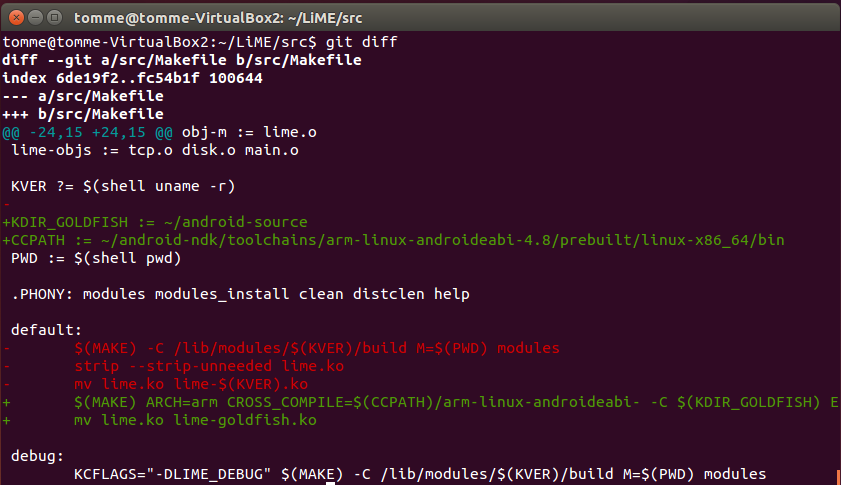
\includegraphics[scale=0.3]{diff.png} \\
  Make the kernel module\\
  \texttt{\justify make} \\
  Push the kernel module to the emulator\\
  \texttt{\justify ~/android-sdk/sdk/platform-tools/adb push ~/LiME/lime-goldfish.ko /sdcard/lime.ko} \\
  Start up a shell on the emulator\\
  \texttt{\justify ~/android-sdk/sdk/platform-tools/adb shell} \\
  In the shell type:\\
  \texttt{\justify insmod /sdcard/lime.ko "path=/sdcard/lime.dump format=lime"} \\
  You now have your memory dump in /sdcard/lime.dump\\
  Transfer it yo your PC and you you can analyse it with volatility or other tools.
  
  

\nocite{*}

% conference papers do not normally have an appendix


% use section* for acknowledgement
%section*{Acknowledgment}


%The authors would like to thank...





% trigger a \newpage just before the given reference
% number - used to balance the columns on the last page
% adjust value as needed - may need to be readjusted if
% the document is modified later
%\IEEEtriggeratref{8}
% The "triggered" command can be changed if desired:
%\IEEEtriggercmd{\enlargethispage{-5in}}

% references section

% can use a bibliography generated by BibTeX as a .bbl file
% BibTeX documentation can be easily obtained at:
% http://www.ctan.org/tex-archive/biblio/bibtex/contrib/doc/
% The IEEEtran BibTeX style support page is at:
% http://www.michaelshell.org/tex/ieeetran/bibtex/
\bibliographystyle{IEEEtran}
% argument is your BibTeX string definitions and bibliography database(s)
\bibliography{IEEEabrv,bib}
%
% <OR> manually copy in the resultant .bbl file
% set second argument of \begin to the number of references
% (used to reserve space for the reference number labels box)




% that's all folks
\end{document}


\grid
